\section{Introduction}
\label{sec:introduction}

In this laboratory assignment we analysed, theoreticaly and also in regards to simulation, a Pass-band Filter using an Operational Amplifier (OPAMP).
This was composed by three stages: a High Pass stage, with the goal of passing high frequencie signals and cutting the ones with a low frequencie, and Amplification stage, where, using the OPAMP, the signals were amplified, and a Low Pass Stage that cuts off high frequency signals and allows the ones with low frequency to pass. For the OPAMP, we chose the model $\mu$A741 from Texas Instruments. In this report we will do first the theoretical analysis, followed by the simulation using NGSpice in \ref{sec:analysis}. In the end of this section we will compare the simulation and the theoratical analysis. The conclusions are presented in \ref{sec:conclusion}.
The stated circuit is presented in \ref{fig:circuitol5}.


\begin{figure}[h] \centering
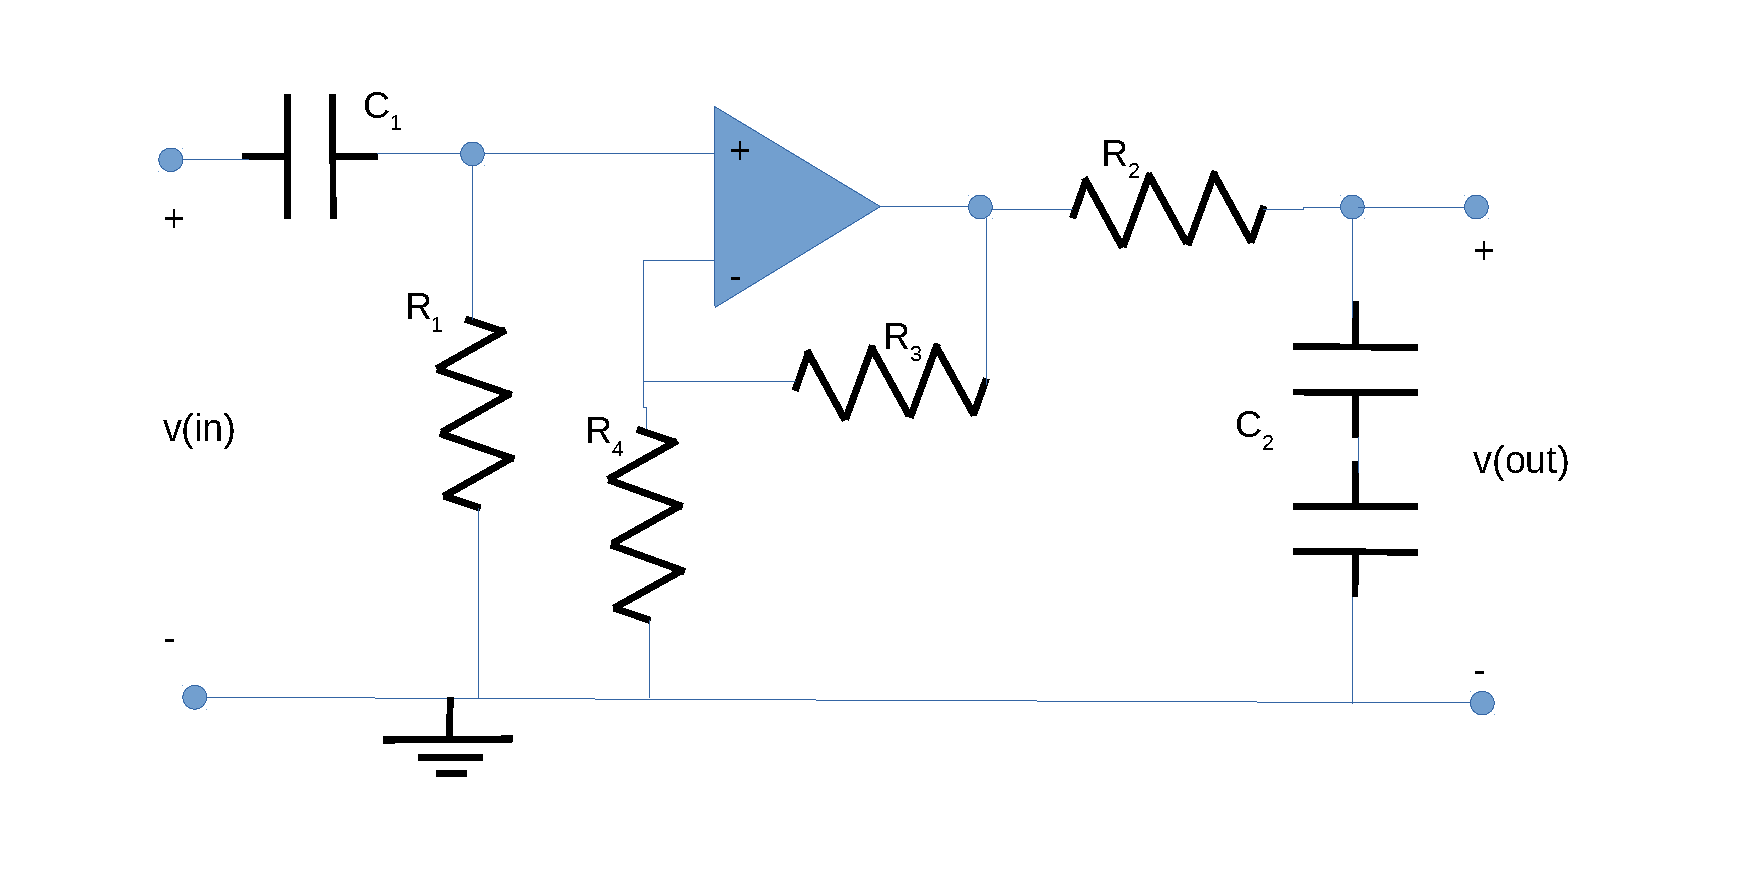
\includegraphics[width=1\linewidth]{circuitl5_old.pdf}
\caption{Active Passband Filter}
\label{fig:circuitol5}
\end{figure}

\clearpage
